\twocolumn[\section{Rules Reference Guide}]
\label{sec:RulesReferenceGuide}

\newreference{Ability bonus}{sec:Abilitybonus}
Many Starting Deck Cards and Upgrade Cards provide an Ability Bonus ( TBD see image), which is considered to be in effect for the rest of the round.

\newreference{Alliance deck}{sec:Alliancedeck}
TBD

\related{sec:Discardpile}

\newreference{Archway}{sec:Archway}
Whenever a hero opens a door (whether it is a normal door, locked door, or secret door) between two Dungeon Tiles, she places an Archway Token between the two tiles to show that the passage is now clear.

There are 30 archway tokens included in the base game.

\related{sec:Dungeontile}

\newreference{Artifacts}{sec:Artifacts}
The Level III Upgrade Deck only has one card type: artifacts. When you draft an artifact, do not place it in your hand as normal. Instead, place the artifact face up on the table beside your Hero Cards. The artifact’s text provides a continuous benefit to all of your heroes. You may acquire multiple artifacts during the course of the game.

\newreference{Attack}{sec:Attack}

There are two types of attacks: melee and ranged . Your hero’s attack strength is listed beside the red Attack Icon on her Hero Card. The Attack Icon also indicates whether or not the hero’s primary attack is melee or ranged

TBD Attack type icons

\textbf{Once your hero has attacked he cannot:}
\begin{itemize}
  \item move again or continue spending remaining speed points
  \item do any other actions like playing cards, opening doors, unlocking chests etc.
\end{itemize}

\related{sec:Attackstrength, sec:Speedpoint}

\index{Attack!Melee attack}
\index{Attack!Ranged attack}

\newreference{Attack strength}{sec:Attackstrength}

There are two types of attacks: melee and ranged . Your hero’s attack
strength is listed beside the red Attack Icon on her Hero Card. The Attack Icon
also indicates whether or not the hero’s primary attack is melee or ranged.
You may also play cards from your hand that are usable by the active hero to
provide additional attack strength for your hero. A card that features the
"+ Melee Attack" icon (see right) adds to your hero’s melee attack total.

A card that features the “+ Ranged Attack” icon (see right) adds to your hero’s
ranged attack strength total.

\newreference{Battle}{sec:Battle}
TBD

\newreference{Basic game}{sec:Basicgame}

\newreference{Burst of Strength}{sec:BurstofStrength}
TBD

\newreference{Campaign}{sec:Campaign}
TBD

\newreference{Card type}{sec:Cardtype}
TBD

\newreference{Challenge}{sec:Challenge}
TBD

\newreference{Challenge token}{sec:Challengetoken}
TBD

\newreference{Champions of Dungeon Alliance}{sec:ChampionsofDungeonAlliance}
TBD

\newreference{Class}{sec:Class}
TBD

\newreference{Combat die}{sec:Combatdie}
\seeonpage{sec:Dungeondie}.

\newreference{Cooperative}{sec:Cooperative}
TBD

\newreference{Cycle}{sec:Cycle}
TBD

\newreference{Damage}{sec:Damage}
TBD

\newreference{Deck of Many Treasures}{sec:DeckofManyTreasures}
TBD

\newreference{Defeat}{sec:Defeat}
TBD

\newreference{Defeated hero}{sec:Defeatedhero}
TBD

\newreference{Determine damage}{sec:Determinedamage}
TBD

\newreference{Disarm}{sec:Disarm}
TBD

\newreference{Disarm trap}{sec:Disarmtrap}
TBD

\newreference{Discard}{sec:Discard}
TBD

\newreference{Discard pile}{sec:Discardpile}
TBD

\newreference{Draft Bonus Chart}{sec:DraftBonusChart}
TBD

\newreference{Draft upgrade}{sec:Draftupgrade}
TBD

\newreference{Draw cards}{sec:Drawcards}
TBD

\newreference{Dungeon die}{sec:Dungeondie}
TBD

\newreference{Dungeon tile}{sec:Dungeontile}
TBD

\begin{table}[H]
%\centering
\resizebox{\columnwidth}{!}{\begin{tabular}{|c|>{\centering\arraybackslash\hspace{0pt}}p{.4cm}|>{\centering\arraybackslash\hspace{0pt}}p{.4cm}|>{\centering\arraybackslash\hspace{0pt}}p{.4cm}|>{\centering\arraybackslash\hspace{0pt}}p{.4cm}|}
\hline
\rowcolor{tableheadcolor}
\color{white}\trajan\fontsize{10}{10}\selectfont\# of Players & \color{white}\trajan\fontsize{10}{10}\selectfont1 & \color{white}\trajan\fontsize{10}{10}\selectfont2 & \color{white}\trajan\fontsize{10}{10}\selectfont3 & \color{white}\trajan\fontsize{10}{10}\selectfont4 \\
\hline
Level I dungeon tile count & 6 & 6 & 8 & 10 \\
\hline
Level II dungeon tile count & 4 & 5 & 6 & 7 \\
\hline
Level III dungeon tile count & 2 & 2 & 3 & 4 \\
\hline
\end{tabular}}
\end{table}

\newreference{Encounter token}{sec:Encountertoken}
TBD

\newreference{End Phase}{sec:EndPhase}

\seeonpage{sec:Gameround}

\newreference{Experience point}{sec:Experiencepoint}

\seeonpage{sec:XP}

\newreference{Game cycle}{sec:Gamecycle}
TBD

\newreference{Game round}{sec:Gameround}
A game of Dungeon alliance consists of four complete rounds. Each round consists of four \myuline{\hyperref[sec:Gamecycle]{game cycles}} and one end phase.

\index{Game round!Hero activation}
\index{Game round!Monster activation}
\index{Game round!End phase}

\newreference{Generic starting deck}{sec:Genericstartingdeck}

Generic starting deck cards (32 cards) are only used in the Basic Game. There are four sets of 8 cards included, one set for each player.

One set consists of:
\begin{itemize}
  \item 2 copies of "Precision Attack"
  \item 2 copies of "Reflex"
  \item 2 copies of "Minor Potion of Healing" and
  \item 2 copies of "Surge Forward"
\end{itemize}

In basic game these are then shuffled with the 4 unique Starting deck cards (the \#1 card from each hero) to form the starting Alliance deck of 12 cards.

\related{sec:Basicgame}

\newreference{Hand size}{sec:Handsize}

Hand size means the amount of cards on your hand. 

The hand size listed in the Draft Bonus Chart is considered to be the suggested minimum hand size rather than the maximum. This means that you can have more cards in your hand at any point and you are not forced to discard any of them. This also means you might not have enough cards to draw at the Discard \& Draw phase of hero activation and thus you need to play remaining hero activations with the limited number of cards until you either draft more cards or form a new discard pile at the end phase of game round.

After you are done discarding cards (or decided not to) at the Discard \& Draw phase of hero activation, you must draw new cards from the top of your Alliance Deck until the number of cards in your hand is equal to your hand size as depicted on your Draft Bonus Chart. If you run out of cards in your Alliance Deck while drawing, shuffle your Alliance Discard Pile to form your new Alliance Deck. If you run out of cards in both your Alliance Deck and its discard pile, then you must play your next Hero Activation with the limited number of cards that you have drawn.

\related{sec:Gameround, sec:Alliancedeck}

\newreference{Hero activation}{sec:Heroactivation}

\seeonpage{sec:Gameround}

\newreference{Hero card}{sec:Herocard}
TBD

\newreference{Hero token}{sec:Herotoken}
TBD

\newreference{Hero vs Hero}{sec:HerovsHero}
TBD

\newreference{Hero vs Monster}{sec:HerovsMonster}
TBD

\newreference{Hourglass icon}{sec:Hourglassicon}
The hourglass icon on the card is a reminder that the card has a text ability that lasts for the rest of the round.

TBD Image

\newreference{Initiative token}{sec:Initiativetoken}
TBD

\newreference{Line of sight}{sec:Lineofsight}
TBD

\newreference{Melee attack}{sec:Meleeattack}

\seeonpage{sec:Attack}.

\newreference{Monster activation}{sec:Monsteractivation}

\seeonpage{sec:Gameround}

\newreference{Monster movement}{sec:Monstermovement}
TBD

\newreference{Monster token}{sec:Monstertoken}
TBD

\newreference{Move hero}{sec:Movehero}
TBD

\newreference{Move monster}{sec:Movemonster}
TBD

\newreference{Movement}{sec:Movement}
TBD

\related{sec:Speedpoint}


\newreference{Nightmare}{sec:Nightmare}
TBD

\newreference{Obstruction defense}{sec:Obstructiondefense}
TBD

\newreference{Permadeath}{sec:Permadeath}
TBD

\newreference{Pet}{sec:Pet}
TBD

\newreference{Quest}{sec:Quest}

\setlength{\columnsep}{2pt}%
\setlength{\intextsep}{2pt}%
\begin{wrapfigure}{r}{.5\columnwidth}
\centering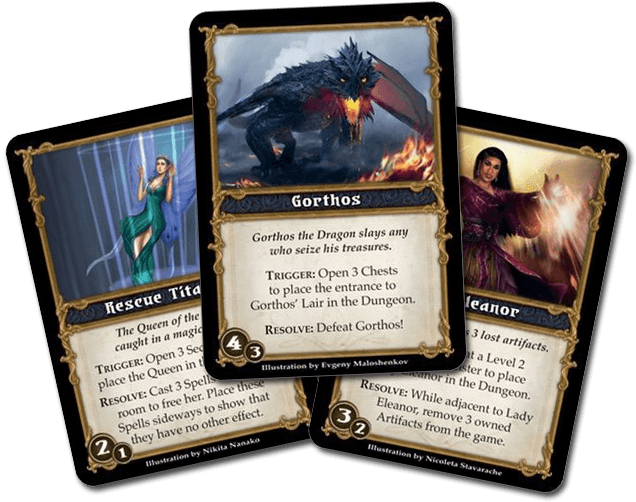
\includegraphics[width=.5\columnwidth]{images/quest_cards.png}
\caption*{Quest cards}
\end{wrapfigure}

Quest Cards give players different level of goals throughout their game. Each Quest Card features a Quest name \refimageannotation{1} and Quest Background \refimageannotation{2} that describes the quest's storyline.

The Quest trigger \refimageannotation{2} is the circumstance that brings the quest's
corresponding \myuline{\hyperref[sec:Questtoken]{Quest Token}} into play. The Quest resolution \refimageannotation{3} is the activity that players must
perform in order to complete the quest after it is in play.

If more than one Dungeon Alliance works together to
accomplish the quest, then the Alliance that contributed the
most toward the Quest's resolution receives the first XP
reward (here 4 XP), and the Alliance that contributed the second most
receives the second XP Reward (here 3 XP). If only one Dungeon Alliance
accomplishes the quest, then that Alliance receives the
combined value of both XP Rewards (here 7 XP) \refimageannotation{5}.

\hfill\begin{tikzpicture}
    \node[anchor=north west,inner sep=0] at (0,0) {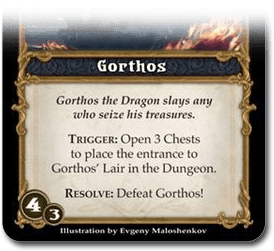
\includegraphics[width=0.6\columnwidth]{images/quest_card_detail_fade.png}};
%    \draw[red,ultra thick,rounded corners] (7.5,5.3) rectangle (9.4,6.2);
    \draw (1.2,-1.3)node[mynode,anchor=west] {1};
    \draw (2.5,-2.2)node[mynode,anchor=west] {2};
    \draw (2.5,-3.0)node[mynode,anchor=west] {3};
    \draw (2.5,-3.9)node[mynode,anchor=west] {4};
    \draw (0.5,-4.5)node[mynode,anchor=west] {5};
    %\draw[step=1cm,gray,very thin] (0,0) grid (6,-6);
\end{tikzpicture}\hspace*{\fill}

\newreference{Quest token}{sec:Questtoken}
TBD

\newreference{Race}{sec:Race}
TBD

\newreference{Ranged attack}{sec:Rangedattack}

\seeonpage{sec:Attack}.

\newreference{Ranged monster}{sec:Rangedmonster}
TBD

\newreference{Ready monster}{sec:Readymonster}
TBD

\newreference{Reference card}{sec:Referencecard}
TBD

\newreference{Rest}{sec:Rest}
TBD

\newreference{Rotation}{sec:Rotation}
TBD

\newreference{Round summary}{sec:Roundsummary}
TBD

\seerulebookpage{13}
\seerulesupplementpage{22}

\newreference{Solo}{sec:Solo}
TBD

\newreference{Solo play}{sec:Soloplay}
TBD

\newreference{Solo/Cooperative card}{sec:SoloCooperativecard}
TBD

\newreference{Special Power}{sec:SpecialPower}
TBD

\newreference{Speed point}{sec:Speedpoint}
TBD

\newreference{Spell}{sec:Spell}
TBD

\newreference{Spin}{sec:Spin}
Hero can spin (i.e. change direction) freely before attacking. After attacking, hero cannot move and therefore cannot also spin anymore.

\newreference{Stairs}{sec:Stairs}
TBD

\newreference{Starting deck}{sec:Startingdeck}
TBD

\newreference{Trap}{sec:Trap}
TBD

\index{Trap!Pit Trap}
\index{Trap!Dart Trap}
\index{Trap!Flame Trap}
\index{Trap!Arrow Wall Trap}
\index{Trap!Lightning Trap}
\index{Trap!Pendulum Trap}

\newreference{Treasure}{sec:Treasure}
TBD

\newreference{Turn}{sec:Turn}
\seeonpage{sec:Spin}

\newreference{Upgrade}{sec:Upgrade}
TBD

\newreference{Upgrade card}{sec:Upgradecard}
TBD

\newreference{Upgrade level}{sec:Upgradelevel}
TBD

\newreference{Winning}{sec:Winning}
TBD

\newreference{Wound}{sec:Wound}
TBD

\newreference{XP}{sec:XP}
TBD

\newreference{XP pool}{sec:XPpool}
TBD
